\documentclass[1p]{elsarticle_modified}
%\bibliographystyle{elsarticle-num}

%\usepackage[colorlinks]{hyperref}
%\usepackage{abbrmath_seonhwa} %\Abb, \Ascr, \Acal ,\Abf, \Afrak
\usepackage{amsfonts}
\usepackage{amssymb}
\usepackage{amsmath}
\usepackage{amsthm}
\usepackage{scalefnt}
\usepackage{amsbsy}
\usepackage{kotex}
\usepackage{caption}
\usepackage{subfig}
\usepackage{color}
\usepackage{graphicx}
\usepackage{xcolor} %% white, black, red, green, blue, cyan, magenta, yellow
\usepackage{float}
\usepackage{setspace}
\usepackage{hyperref}

\usepackage{tikz}
\usetikzlibrary{arrows}

\usepackage{multirow}
\usepackage{array} % fixed length table
\usepackage{hhline}

%%%%%%%%%%%%%%%%%%%%%
\makeatletter
\renewcommand*\env@matrix[1][\arraystretch]{%
	\edef\arraystretch{#1}%
	\hskip -\arraycolsep
	\let\@ifnextchar\new@ifnextchar
	\array{*\c@MaxMatrixCols c}}
\makeatother %https://tex.stackexchange.com/questions/14071/how-can-i-increase-the-line-spacing-in-a-matrix
%%%%%%%%%%%%%%%

\usepackage[normalem]{ulem}

\newcommand{\msout}[1]{\ifmmode\text{\sout{\ensuremath{#1}}}\else\sout{#1}\fi}
%SOURCE: \msout is \stkout macro in https://tex.stackexchange.com/questions/20609/strikeout-in-math-mode

\newcommand{\cancel}[1]{
	\ifmmode
	{\color{red}\msout{#1}}
	\else
	{\color{red}\sout{#1}}
	\fi
}

\newcommand{\add}[1]{
	{\color{blue}\uwave{#1}}
}

\newcommand{\replace}[2]{
	\ifmmode
	{\color{red}\msout{#1}}{\color{blue}\uwave{#2}}
	\else
	{\color{red}\sout{#1}}{\color{blue}\uwave{#2}}
	\fi
}

\newcommand{\Sol}{\mathcal{S}} %segment
\newcommand{\D}{D} %diagram
\newcommand{\A}{\mathcal{A}} %arc


%%%%%%%%%%%%%%%%%%%%%%%%%%%%%5 test

\def\sl{\operatorname{\textup{SL}}(2,\Cbb)}
\def\psl{\operatorname{\textup{PSL}}(2,\Cbb)}
\def\quan{\mkern 1mu \triangleright \mkern 1mu}

\theoremstyle{definition}
\newtheorem{thm}{Theorem}[section]
\newtheorem{prop}[thm]{Proposition}
\newtheorem{lem}[thm]{Lemma}
\newtheorem{ques}[thm]{Question}
\newtheorem{cor}[thm]{Corollary}
\newtheorem{defn}[thm]{Definition}
\newtheorem{exam}[thm]{Example}
\newtheorem{rmk}[thm]{Remark}
\newtheorem{alg}[thm]{Algorithm}

\newcommand{\I}{\sqrt{-1}}
\begin{document}

%\begin{frontmatter}
%
%\title{Boundary parabolic representations of knots up to 8 crossings}
%
%%% Group authors per affiliation:
%\author{Yunhi Cho} 
%\address{Department of Mathematics, University of Seoul, Seoul, Korea}
%\ead{yhcho@uos.ac.kr}
%
%
%\author{Seonhwa Kim} %\fnref{s_kim}}
%\address{Center for Geometry and Physics, Institute for Basic Science, Pohang, 37673, Korea}
%\ead{ryeona17@ibs.re.kr}
%
%\author{Hyuk Kim}
%\address{Department of Mathematical Sciences, Seoul National University, Seoul 08826, Korea}
%\ead{hyukkim@snu.ac.kr}
%
%\author{Seokbeom Yoon}
%\address{Department of Mathematical Sciences, Seoul National University, Seoul, 08826,  Korea}
%\ead{sbyoon15@snu.ac.kr}
%
%\begin{abstract}
%We find all boundary parabolic representation of knots up to 8 crossings.
%
%\end{abstract}
%\begin{keyword}
%    \MSC[2010] 57M25 
%\end{keyword}
%
%\end{frontmatter}

%\linenumbers
%\tableofcontents
%
\newcommand\colored[1]{\textcolor{white}{\rule[-0.35ex]{0.8em}{1.4ex}}\kern-0.8em\color{red} #1}%
%\newcommand\colored[1]{\textcolor{white}{ #1}\kern-2.17ex	\textcolor{white}{ #1}\kern-1.81ex	\textcolor{white}{ #1}\kern-2.15ex\color{red}#1	}

{\Large $\underline{12n_{0534}~(K12n_{0534})}$}

\setlength{\tabcolsep}{10pt}
\renewcommand{\arraystretch}{1.6}
\vspace{1cm}\begin{tabular}{m{100pt}>{\centering\arraybackslash}m{274pt}}
\multirow{5}{120pt}{
	\centering
	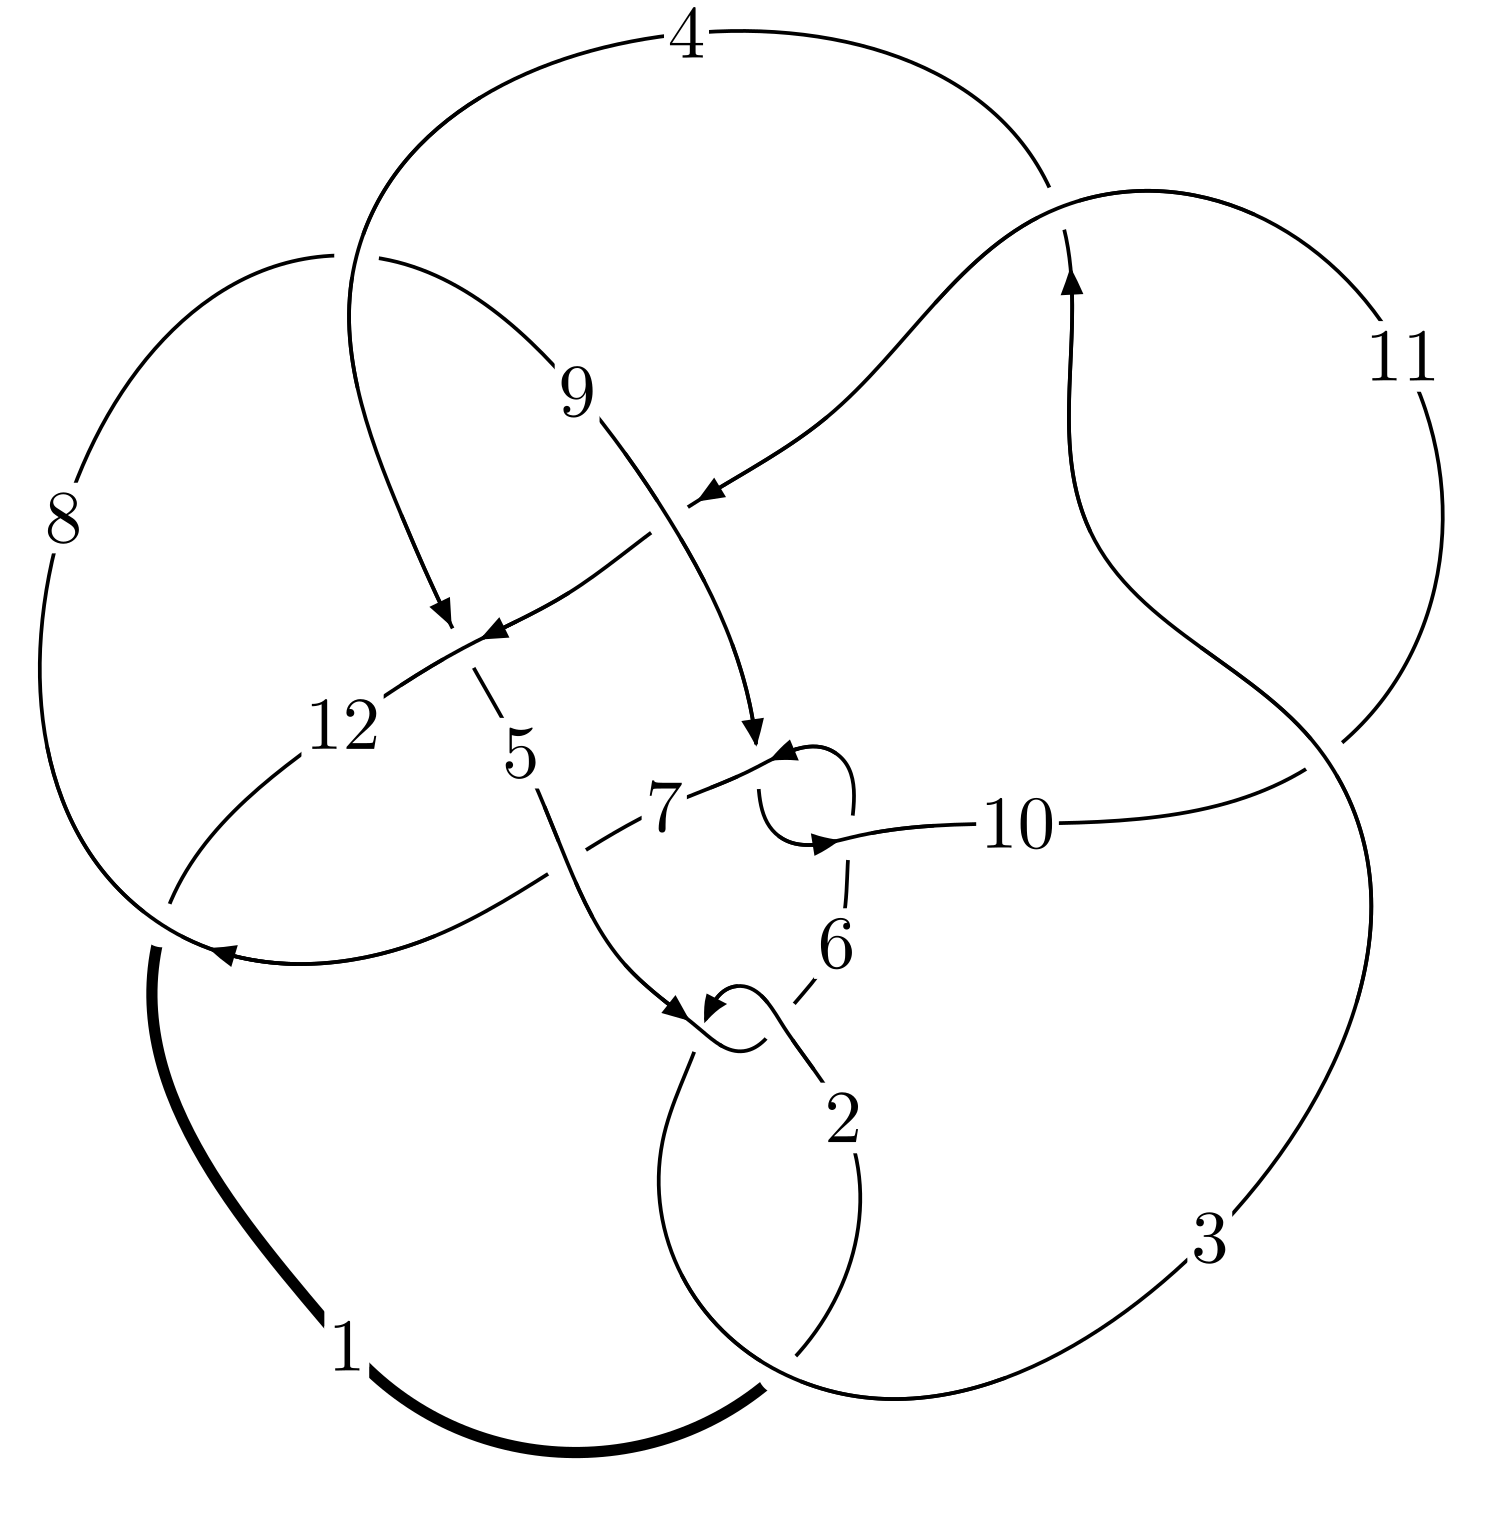
\includegraphics[width=112pt]{../../../GIT/diagram.site/Diagrams/png/2623_12n_0534.png}\\
\ \ \ A knot diagram\footnotemark}&
\allowdisplaybreaks
\textbf{Linearized knot diagam} \\
\cline{2-2}
 &
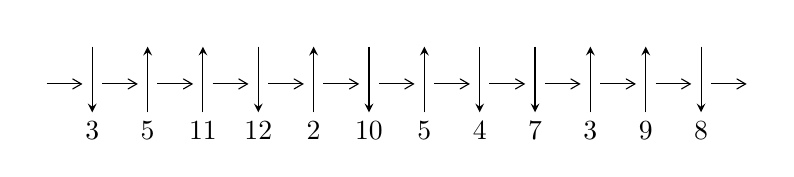
\begin{tikzpicture}[x=20pt, y=17pt]
	% nodes
	\node (C0) at (0, 0) {};
	\node (C1) at (1, 0) {};
	\node (C1U) at (1, +1) {};
	\node (C1D) at (1, -1) {3};

	\node (C2) at (2, 0) {};
	\node (C2U) at (2, +1) {};
	\node (C2D) at (2, -1) {5};

	\node (C3) at (3, 0) {};
	\node (C3U) at (3, +1) {};
	\node (C3D) at (3, -1) {11};

	\node (C4) at (4, 0) {};
	\node (C4U) at (4, +1) {};
	\node (C4D) at (4, -1) {12};

	\node (C5) at (5, 0) {};
	\node (C5U) at (5, +1) {};
	\node (C5D) at (5, -1) {2};

	\node (C6) at (6, 0) {};
	\node (C6U) at (6, +1) {};
	\node (C6D) at (6, -1) {10};

	\node (C7) at (7, 0) {};
	\node (C7U) at (7, +1) {};
	\node (C7D) at (7, -1) {5};

	\node (C8) at (8, 0) {};
	\node (C8U) at (8, +1) {};
	\node (C8D) at (8, -1) {4};

	\node (C9) at (9, 0) {};
	\node (C9U) at (9, +1) {};
	\node (C9D) at (9, -1) {7};

	\node (C10) at (10, 0) {};
	\node (C10U) at (10, +1) {};
	\node (C10D) at (10, -1) {3};

	\node (C11) at (11, 0) {};
	\node (C11U) at (11, +1) {};
	\node (C11D) at (11, -1) {9};

	\node (C12) at (12, 0) {};
	\node (C12U) at (12, +1) {};
	\node (C12D) at (12, -1) {8};
	\node (C13) at (13, 0) {};

	% arrows
	\draw[->,>={angle 60}]
	(C0) edge (C1) (C1) edge (C2) (C2) edge (C3) (C3) edge (C4) (C4) edge (C5) (C5) edge (C6) (C6) edge (C7) (C7) edge (C8) (C8) edge (C9) (C9) edge (C10) (C10) edge (C11) (C11) edge (C12) (C12) edge (C13) ;	\draw[->,>=stealth]
	(C1U) edge (C1D) (C2D) edge (C2U) (C3D) edge (C3U) (C4U) edge (C4D) (C5D) edge (C5U) (C6U) edge (C6D) (C7D) edge (C7U) (C8U) edge (C8D) (C9U) edge (C9D) (C10D) edge (C10U) (C11D) edge (C11U) (C12U) edge (C12D) ;
	\end{tikzpicture} \\
\hhline{~~} \\& 
\textbf{Solving Sequence} \\ \cline{2-2} 
 &
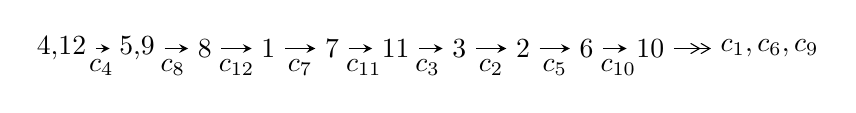
\begin{tikzpicture}[x=23pt, y=7pt]
	% node
	\node (A0) at (-1/8, 0) {4,12};
	\node (A1) at (17/16, 0) {5,9};
	\node (A2) at (17/8, 0) {8};
	\node (A3) at (25/8, 0) {1};
	\node (A4) at (33/8, 0) {7};
	\node (A5) at (41/8, 0) {11};
	\node (A6) at (49/8, 0) {3};
	\node (A7) at (57/8, 0) {2};
	\node (A8) at (65/8, 0) {6};
	\node (A9) at (73/8, 0) {10};
	\node (C1) at (1/2, -1) {$c_{4}$};
	\node (C2) at (13/8, -1) {$c_{8}$};
	\node (C3) at (21/8, -1) {$c_{12}$};
	\node (C4) at (29/8, -1) {$c_{7}$};
	\node (C5) at (37/8, -1) {$c_{11}$};
	\node (C6) at (45/8, -1) {$c_{3}$};
	\node (C7) at (53/8, -1) {$c_{2}$};
	\node (C8) at (61/8, -1) {$c_{5}$};
	\node (C9) at (69/8, -1) {$c_{10}$};
	\node (A10) at (11, 0) {$c_{1},c_{6},c_{9}$};

	% edge
	\draw[->,>=stealth]	
	(A0) edge (A1) (A1) edge (A2) (A2) edge (A3) (A3) edge (A4) (A4) edge (A5) (A5) edge (A6) (A6) edge (A7) (A7) edge (A8) (A8) edge (A9) ;
	\draw[->>,>={angle 60}]	
	(A9) edge (A10);
\end{tikzpicture} \\ 

\end{tabular} \\

\footnotetext{
The image of knot diagram is generated by the software ``\textbf{Draw programme}" developed by Andrew Bartholomew(\url{http://www.layer8.co.uk/maths/draw/index.htm\#Running-draw}), where we modified some parts for our purpose(\url{https://github.com/CATsTAILs/LinksPainter}).
}\phantom \\ \newline 
\centering \textbf{Ideals for irreducible components\footnotemark of $X_{\text{par}}$} 
 
\begin{align*}
I^u_{1}&=\langle 
-3.69906\times10^{250} u^{76}-1.26904\times10^{251} u^{75}+\cdots+6.74175\times10^{250} b-1.48767\times10^{251},\\
\phantom{I^u_{1}}&\phantom{= \langle  }-2.19520\times10^{251} u^{76}-8.95593\times10^{251} u^{75}+\cdots+6.74175\times10^{250} a-1.13911\times10^{252},\\
\phantom{I^u_{1}}&\phantom{= \langle  }u^{77}+4 u^{76}+\cdots+14 u+1\rangle \\
I^u_{2}&=\langle 
-9.09164\times10^{21} u^{22}+3.04025\times10^{21} u^{21}+\cdots+1.47737\times10^{22} b+1.58364\times10^{22},\\
\phantom{I^u_{2}}&\phantom{= \langle  }-1.26080\times10^{22} u^{22}+3.40886\times10^{22} u^{21}+\cdots+7.38683\times10^{22} a-5.26178\times10^{22},\;u^{23}- u^{22}+\cdots- u+1\rangle \\
\\
\end{align*}
\raggedright * 2 irreducible components of $\dim_{\mathbb{C}}=0$, with total 100 representations.\\
\footnotetext{All coefficients of polynomials are rational numbers. But the coefficients are sometimes approximated in decimal forms when there is not enough margin.}
\newpage
\renewcommand{\arraystretch}{1}
\centering \section*{I. $I^u_{1}= \langle -3.70\times10^{250} u^{76}-1.27\times10^{251} u^{75}+\cdots+6.74\times10^{250} b-1.49\times10^{251},\;-2.20\times10^{251} u^{76}-8.96\times10^{251} u^{75}+\cdots+6.74\times10^{250} a-1.14\times10^{252},\;u^{77}+4 u^{76}+\cdots+14 u+1 \rangle$}
\flushleft \textbf{(i) Arc colorings}\\
\begin{tabular}{m{7pt} m{180pt} m{7pt} m{180pt} }
\flushright $a_{4}=$&$\begin{pmatrix}1\\0\end{pmatrix}$ \\
\flushright $a_{12}=$&$\begin{pmatrix}0\\u\end{pmatrix}$ \\
\flushright $a_{5}=$&$\begin{pmatrix}1\\u^2\end{pmatrix}$ \\
\flushright $a_{9}=$&$\begin{pmatrix}3.25613 u^{76}+13.2843 u^{75}+\cdots+159.304 u+16.8963\\0.548680 u^{76}+1.88235 u^{75}+\cdots+31.3932 u+2.20665\end{pmatrix}$ \\
\flushright $a_{8}=$&$\begin{pmatrix}3.80481 u^{76}+15.1666 u^{75}+\cdots+190.697 u+19.1029\\0.548680 u^{76}+1.88235 u^{75}+\cdots+31.3932 u+2.20665\end{pmatrix}$ \\
\flushright $a_{1}=$&$\begin{pmatrix}3.72053 u^{76}+15.8998 u^{75}+\cdots+60.2006 u-1.37429\\0.115206 u^{76}+0.587561 u^{75}+\cdots-5.69859 u-1.78085\end{pmatrix}$ \\
\flushright $a_{7}=$&$\begin{pmatrix}2.99371 u^{76}+12.2116 u^{75}+\cdots+156.235 u+16.9489\\0.442657 u^{76}+1.58355 u^{75}+\cdots+28.1540 u+1.91734\end{pmatrix}$ \\
\flushright $a_{11}=$&$\begin{pmatrix}2.87213 u^{76}+12.3222 u^{75}+\cdots+75.2678 u+2.03206\\0.733192 u^{76}+2.99004 u^{75}+\cdots-7.36863 u-1.62550\end{pmatrix}$ \\
\flushright $a_{3}=$&$\begin{pmatrix}0.590451 u^{76}+3.55470 u^{75}+\cdots+32.3369 u+12.2851\\0.0782665 u^{76}+0.462570 u^{75}+\cdots+25.4892 u+3.43765\end{pmatrix}$ \\
\flushright $a_{2}=$&$\begin{pmatrix}0.681023 u^{76}+4.03467 u^{75}+\cdots-10.4432 u+7.65451\\0.255746 u^{76}+1.13089 u^{75}+\cdots+23.7511 u+3.31997\end{pmatrix}$ \\
\flushright $a_{6}=$&$\begin{pmatrix}-2.01550 u^{76}-7.43009 u^{75}+\cdots-246.167 u-23.7129\\-0.454144 u^{76}-1.61501 u^{75}+\cdots-39.0367 u-2.17934\end{pmatrix}$ \\
\flushright $a_{10}=$&$\begin{pmatrix}4.72922 u^{76}+19.1431 u^{75}+\cdots+210.364 u+20.7645\\1.01772 u^{76}+4.07896 u^{75}+\cdots+27.5236 u+1.58371\end{pmatrix}$\\&\end{tabular}
\flushleft \textbf{(ii) Obstruction class $= -1$}\\~\\
\flushleft \textbf{(iii) Cusp Shapes $= -2.26612 u^{76}-10.0790 u^{75}+\cdots-56.7965 u-6.97634$}\\~\\
\newpage\renewcommand{\arraystretch}{1}
\flushleft \textbf{(iv) u-Polynomials at the component}\newline \\
\begin{tabular}{m{50pt}|m{274pt}}
Crossings & \hspace{64pt}u-Polynomials at each crossing \\
\hline $$\begin{aligned}c_{1}\end{aligned}$$&$\begin{aligned}
&u^{77}+84 u^{76}+\cdots+220776 u-9409
\end{aligned}$\\
\hline $$\begin{aligned}c_{2},c_{5}\end{aligned}$$&$\begin{aligned}
&u^{77}-2 u^{76}+\cdots+584 u+97
\end{aligned}$\\
\hline $$\begin{aligned}c_{3},c_{10}\end{aligned}$$&$\begin{aligned}
&u^{77}- u^{76}+\cdots-404 u-44
\end{aligned}$\\
\hline $$\begin{aligned}c_{4}\end{aligned}$$&$\begin{aligned}
&u^{77}+4 u^{76}+\cdots+14 u+1
\end{aligned}$\\
\hline $$\begin{aligned}c_{6},c_{9}\end{aligned}$$&$\begin{aligned}
&u^{77}+6 u^{76}+\cdots-8 u+1
\end{aligned}$\\
\hline $$\begin{aligned}c_{7}\end{aligned}$$&$\begin{aligned}
&u^{77}+14 u^{76}+\cdots+936770 u-675287
\end{aligned}$\\
\hline $$\begin{aligned}c_{8}\end{aligned}$$&$\begin{aligned}
&u^{77}+4 u^{76}+\cdots-24 u+1
\end{aligned}$\\
\hline $$\begin{aligned}c_{11}\end{aligned}$$&$\begin{aligned}
&u^{77}-2 u^{76}+\cdots+16 u+1
\end{aligned}$\\
\hline $$\begin{aligned}c_{12}\end{aligned}$$&$\begin{aligned}
&u^{77}-3 u^{76}+\cdots-482672 u+37636
\end{aligned}$\\
\hline
\end{tabular}\\~\\
\newpage\renewcommand{\arraystretch}{1}
\flushleft \textbf{(v) Riley Polynomials at the component}\newline \\
\begin{tabular}{m{50pt}|m{274pt}}
Crossings & \hspace{64pt}Riley Polynomials at each crossing \\
\hline $$\begin{aligned}c_{1}\end{aligned}$$&$\begin{aligned}
&y^{77}-172 y^{76}+\cdots+7173569444 y-88529281
\end{aligned}$\\
\hline $$\begin{aligned}c_{2},c_{5}\end{aligned}$$&$\begin{aligned}
&y^{77}+84 y^{76}+\cdots+220776 y-9409
\end{aligned}$\\
\hline $$\begin{aligned}c_{3},c_{10}\end{aligned}$$&$\begin{aligned}
&y^{77}-37 y^{76}+\cdots+117808 y-1936
\end{aligned}$\\
\hline $$\begin{aligned}c_{4}\end{aligned}$$&$\begin{aligned}
&y^{77}-12 y^{76}+\cdots+68 y-1
\end{aligned}$\\
\hline $$\begin{aligned}c_{6},c_{9}\end{aligned}$$&$\begin{aligned}
&y^{77}+12 y^{76}+\cdots+4 y-1
\end{aligned}$\\
\hline $$\begin{aligned}c_{7}\end{aligned}$$&$\begin{aligned}
&y^{77}+40 y^{76}+\cdots+11472934223744 y-456012532369
\end{aligned}$\\
\hline $$\begin{aligned}c_{8}\end{aligned}$$&$\begin{aligned}
&y^{77}+12 y^{76}+\cdots+98 y-1
\end{aligned}$\\
\hline $$\begin{aligned}c_{11}\end{aligned}$$&$\begin{aligned}
&y^{77}-8 y^{76}+\cdots+54 y-1
\end{aligned}$\\
\hline $$\begin{aligned}c_{12}\end{aligned}$$&$\begin{aligned}
&y^{77}-13 y^{76}+\cdots+29073057280 y-1416468496
\end{aligned}$\\
\hline
\end{tabular}\\~\\
\newpage\flushleft \textbf{(vi) Complex Volumes and Cusp Shapes}
$$\begin{array}{c|c|c}  
\text{Solutions to }I^u_{1}& \I (\text{vol} + \sqrt{-1}CS) & \text{Cusp shape}\\
 \hline 
\begin{aligned}
u &= \phantom{-}0.603067 + 0.813111 I \\
a &= \phantom{-}0.017137 - 1.292070 I \\
b &= \phantom{-}0.99462 + 1.26439 I\end{aligned}
 & \phantom{-}7.23108 - 4.64101 I & \phantom{-0.000000 } 0 \\ \hline\begin{aligned}
u &= \phantom{-}0.603067 - 0.813111 I \\
a &= \phantom{-}0.017137 + 1.292070 I \\
b &= \phantom{-}0.99462 - 1.26439 I\end{aligned}
 & \phantom{-}7.23108 + 4.64101 I & \phantom{-0.000000 } 0 \\ \hline\begin{aligned}
u &= \phantom{-}0.759653 + 0.620579 I \\
a &= -0.729094 + 0.411957 I \\
b &= \phantom{-}0.154848 - 0.382079 I\end{aligned}
 & \phantom{-}1.70009 + 0.34267 I & \phantom{-0.000000 } 0 \\ \hline\begin{aligned}
u &= \phantom{-}0.759653 - 0.620579 I \\
a &= -0.729094 - 0.411957 I \\
b &= \phantom{-}0.154848 + 0.382079 I\end{aligned}
 & \phantom{-}1.70009 - 0.34267 I & \phantom{-0.000000 } 0 \\ \hline\begin{aligned}
u &= -0.572007 + 0.704963 I \\
a &= -0.141969 - 0.535912 I \\
b &= \phantom{-}0.819778 + 1.087240 I\end{aligned}
 & \phantom{-}1.37989 + 3.40941 I & \phantom{-0.000000 } 0. - 7.37735 I \\ \hline\begin{aligned}
u &= -0.572007 - 0.704963 I \\
a &= -0.141969 + 0.535912 I \\
b &= \phantom{-}0.819778 - 1.087240 I\end{aligned}
 & \phantom{-}1.37989 - 3.40941 I & \phantom{-0.000000 -}0. + 7.37735 I \\ \hline\begin{aligned}
u &= -0.876447 + 0.065089 I \\
a &= \phantom{-}1.12695 - 1.60083 I \\
b &= \phantom{-}0.362810 - 0.282958 I\end{aligned}
 & -7.40774 - 0.19172 I & -6.59818 + 0. I\phantom{ +0.000000I} \\ \hline\begin{aligned}
u &= -0.876447 - 0.065089 I \\
a &= \phantom{-}1.12695 + 1.60083 I \\
b &= \phantom{-}0.362810 + 0.282958 I\end{aligned}
 & -7.40774 + 0.19172 I & -6.59818 + 0. I\phantom{ +0.000000I} \\ \hline\begin{aligned}
u &= -0.504176 + 1.001760 I \\
a &= -0.125990 + 1.267870 I \\
b &= \phantom{-}0.534856 - 0.760961 I\end{aligned}
 & \phantom{-}2.41956 + 2.16164 I & \phantom{-0.000000 } 0 \\ \hline\begin{aligned}
u &= -0.504176 - 1.001760 I \\
a &= -0.125990 - 1.267870 I \\
b &= \phantom{-}0.534856 + 0.760961 I\end{aligned}
 & \phantom{-}2.41956 - 2.16164 I & \phantom{-0.000000 } 0\\
 \hline 
 \end{array}$$\newpage$$\begin{array}{c|c|c}  
\text{Solutions to }I^u_{1}& \I (\text{vol} + \sqrt{-1}CS) & \text{Cusp shape}\\
 \hline 
\begin{aligned}
u &= \phantom{-}0.738185 + 0.849245 I \\
a &= -0.975432 + 0.272990 I \\
b &= \phantom{-}0.011881 - 0.595265 I\end{aligned}
 & \phantom{-}2.30258 + 0.23661 I & \phantom{-0.000000 } 0 \\ \hline\begin{aligned}
u &= \phantom{-}0.738185 - 0.849245 I \\
a &= -0.975432 - 0.272990 I \\
b &= \phantom{-}0.011881 + 0.595265 I\end{aligned}
 & \phantom{-}2.30258 - 0.23661 I & \phantom{-0.000000 } 0 \\ \hline\begin{aligned}
u &= -0.851789\phantom{ +0.000000I} \\
a &= -1.52171\phantom{ +0.000000I} \\
b &= -0.970413\phantom{ +0.000000I}\end{aligned}
 & -1.09740\phantom{ +0.000000I} & -10.3570\phantom{ +0.000000I} \\ \hline\begin{aligned}
u &= \phantom{-}0.807485 + 0.037889 I \\
a &= \phantom{-}2.03423 + 0.82063 I \\
b &= \phantom{-}1.039560 - 0.013041 I\end{aligned}
 & -7.69102 + 5.64820 I & -7.22889 - 4.04366 I \\ \hline\begin{aligned}
u &= \phantom{-}0.807485 - 0.037889 I \\
a &= \phantom{-}2.03423 - 0.82063 I \\
b &= \phantom{-}1.039560 + 0.013041 I\end{aligned}
 & -7.69102 - 5.64820 I & -7.22889 + 4.04366 I \\ \hline\begin{aligned}
u &= -0.770876 + 0.163386 I \\
a &= \phantom{-}0.122882 - 1.183720 I \\
b &= \phantom{-}0.62353 + 1.85061 I\end{aligned}
 & -6.89705 - 5.46417 I & -7.68374 + 2.64434 I \\ \hline\begin{aligned}
u &= -0.770876 - 0.163386 I \\
a &= \phantom{-}0.122882 + 1.183720 I \\
b &= \phantom{-}0.62353 - 1.85061 I\end{aligned}
 & -6.89705 + 5.46417 I & -7.68374 - 2.64434 I \\ \hline\begin{aligned}
u &= -0.606094 + 0.481066 I \\
a &= -2.49603 + 0.49755 I \\
b &= -0.334450 + 0.491812 I\end{aligned}
 & -6.05313 + 8.15976 I & -1.59925 - 11.05556 I \\ \hline\begin{aligned}
u &= -0.606094 - 0.481066 I \\
a &= -2.49603 - 0.49755 I \\
b &= -0.334450 - 0.491812 I\end{aligned}
 & -6.05313 - 8.15976 I & -1.59925 + 11.05556 I \\ \hline\begin{aligned}
u &= \phantom{-}0.621201 + 0.435972 I \\
a &= -1.90399 + 0.94577 I \\
b &= -1.049600 - 0.524445 I\end{aligned}
 & -6.07059 - 3.11661 I & -2.10448 + 5.82107 I\\
 \hline 
 \end{array}$$\newpage$$\begin{array}{c|c|c}  
\text{Solutions to }I^u_{1}& \I (\text{vol} + \sqrt{-1}CS) & \text{Cusp shape}\\
 \hline 
\begin{aligned}
u &= \phantom{-}0.621201 - 0.435972 I \\
a &= -1.90399 - 0.94577 I \\
b &= -1.049600 + 0.524445 I\end{aligned}
 & -6.07059 + 3.11661 I & -2.10448 - 5.82107 I \\ \hline\begin{aligned}
u &= \phantom{-}0.748499 + 0.117674 I \\
a &= -0.319645 + 0.370992 I \\
b &= \phantom{-}1.66519 - 1.15111 I\end{aligned}
 & -6.75237 + 0.75022 I & -7.29921 + 3.68885 I \\ \hline\begin{aligned}
u &= \phantom{-}0.748499 - 0.117674 I \\
a &= -0.319645 - 0.370992 I \\
b &= \phantom{-}1.66519 + 1.15111 I\end{aligned}
 & -6.75237 - 0.75022 I & -7.29921 - 3.68885 I \\ \hline\begin{aligned}
u &= -0.523660 + 0.493433 I \\
a &= -0.26799 - 2.25574 I \\
b &= -0.842541 + 0.974175 I\end{aligned}
 & \phantom{-}5.54248 + 3.96289 I & -2.44446 - 3.78941 I \\ \hline\begin{aligned}
u &= -0.523660 - 0.493433 I \\
a &= -0.26799 + 2.25574 I \\
b &= -0.842541 - 0.974175 I\end{aligned}
 & \phantom{-}5.54248 - 3.96289 I & -2.44446 + 3.78941 I \\ \hline\begin{aligned}
u &= -0.465307 + 1.214150 I \\
a &= \phantom{-}0.211228 + 0.623389 I \\
b &= \phantom{-}0.398293 - 0.592596 I\end{aligned}
 & \phantom{-}2.39163 + 1.28478 I & \phantom{-0.000000 } 0 \\ \hline\begin{aligned}
u &= -0.465307 - 1.214150 I \\
a &= \phantom{-}0.211228 - 0.623389 I \\
b &= \phantom{-}0.398293 + 0.592596 I\end{aligned}
 & \phantom{-}2.39163 - 1.28478 I & \phantom{-0.000000 } 0 \\ \hline\begin{aligned}
u &= -0.696063 + 0.006993 I \\
a &= -0.274649 - 0.181788 I \\
b &= -1.096560 + 0.119297 I\end{aligned}
 & -1.55465 + 0.00820 I & -7.37344 + 0.46182 I \\ \hline\begin{aligned}
u &= -0.696063 - 0.006993 I \\
a &= -0.274649 + 0.181788 I \\
b &= -1.096560 - 0.119297 I\end{aligned}
 & -1.55465 - 0.00820 I & -7.37344 - 0.46182 I \\ \hline\begin{aligned}
u &= -0.495506 + 0.487466 I \\
a &= -0.42509 + 1.42469 I \\
b &= -0.27362 - 1.79611 I\end{aligned}
 & -5.63283 + 2.58512 I & -1.14489 - 6.76714 I\\
 \hline 
 \end{array}$$\newpage$$\begin{array}{c|c|c}  
\text{Solutions to }I^u_{1}& \I (\text{vol} + \sqrt{-1}CS) & \text{Cusp shape}\\
 \hline 
\begin{aligned}
u &= -0.495506 - 0.487466 I \\
a &= -0.42509 - 1.42469 I \\
b &= -0.27362 + 1.79611 I\end{aligned}
 & -5.63283 - 2.58512 I & -1.14489 + 6.76714 I \\ \hline\begin{aligned}
u &= -0.988561 + 0.880973 I \\
a &= -0.220670 - 0.465255 I \\
b &= -0.492990 + 1.062540 I\end{aligned}
 & -0.83889 + 3.23068 I & \phantom{-0.000000 } 0 \\ \hline\begin{aligned}
u &= -0.988561 - 0.880973 I \\
a &= -0.220670 + 0.465255 I \\
b &= -0.492990 - 1.062540 I\end{aligned}
 & -0.83889 - 3.23068 I & \phantom{-0.000000 } 0 \\ \hline\begin{aligned}
u &= -0.387945 + 1.272310 I \\
a &= \phantom{-}0.621655 + 0.392644 I \\
b &= -0.651425 - 0.826090 I\end{aligned}
 & -4.61492 - 2.02556 I & \phantom{-0.000000 } 0 \\ \hline\begin{aligned}
u &= -0.387945 - 1.272310 I \\
a &= \phantom{-}0.621655 - 0.392644 I \\
b &= -0.651425 + 0.826090 I\end{aligned}
 & -4.61492 + 2.02556 I & \phantom{-0.000000 } 0 \\ \hline\begin{aligned}
u &= \phantom{-}0.935566 + 0.966645 I \\
a &= -0.002676 + 1.200680 I \\
b &= -0.682271 - 1.007510 I\end{aligned}
 & \phantom{-}1.44567 - 6.72870 I & \phantom{-0.000000 } 0 \\ \hline\begin{aligned}
u &= \phantom{-}0.935566 - 0.966645 I \\
a &= -0.002676 - 1.200680 I \\
b &= -0.682271 + 1.007510 I\end{aligned}
 & \phantom{-}1.44567 + 6.72870 I & \phantom{-0.000000 } 0 \\ \hline\begin{aligned}
u &= -1.089730 + 0.793182 I \\
a &= \phantom{-}0.216148 + 1.161190 I \\
b &= \phantom{-}1.16755 - 1.12635 I\end{aligned}
 & -6.58540 + 8.60086 I & \phantom{-0.000000 } 0 \\ \hline\begin{aligned}
u &= -1.089730 - 0.793182 I \\
a &= \phantom{-}0.216148 - 1.161190 I \\
b &= \phantom{-}1.16755 + 1.12635 I\end{aligned}
 & -6.58540 - 8.60086 I & \phantom{-0.000000 } 0 \\ \hline\begin{aligned}
u &= \phantom{-}0.494600 + 0.409927 I \\
a &= \phantom{-}0.195116 - 0.713007 I \\
b &= -1.83684 + 1.39416 I\end{aligned}
 & -6.21653 - 7.51366 I & -3.0342 + 15.2771 I\\
 \hline 
 \end{array}$$\newpage$$\begin{array}{c|c|c}  
\text{Solutions to }I^u_{1}& \I (\text{vol} + \sqrt{-1}CS) & \text{Cusp shape}\\
 \hline 
\begin{aligned}
u &= \phantom{-}0.494600 - 0.409927 I \\
a &= \phantom{-}0.195116 + 0.713007 I \\
b &= -1.83684 - 1.39416 I\end{aligned}
 & -6.21653 + 7.51366 I & -3.0342 - 15.2771 I \\ \hline\begin{aligned}
u &= \phantom{-}0.559470 + 0.256633 I \\
a &= \phantom{-}0.25535 + 1.85165 I \\
b &= \phantom{-}0.101923 - 0.706888 I\end{aligned}
 & -0.67022 - 2.58077 I & -5.47128 - 2.25816 I \\ \hline\begin{aligned}
u &= \phantom{-}0.559470 - 0.256633 I \\
a &= \phantom{-}0.25535 - 1.85165 I \\
b &= \phantom{-}0.101923 + 0.706888 I\end{aligned}
 & -0.67022 + 2.58077 I & -5.47128 + 2.25816 I \\ \hline\begin{aligned}
u &= \phantom{-}0.545951 + 0.227105 I \\
a &= \phantom{-}1.73598 + 2.22492 I \\
b &= \phantom{-}0.315590 + 0.060991 I\end{aligned}
 & -0.83120 - 2.98976 I & -7.50848 + 10.23936 I \\ \hline\begin{aligned}
u &= \phantom{-}0.545951 - 0.227105 I \\
a &= \phantom{-}1.73598 - 2.22492 I \\
b &= \phantom{-}0.315590 - 0.060991 I\end{aligned}
 & -0.83120 + 2.98976 I & -7.50848 - 10.23936 I \\ \hline\begin{aligned}
u &= \phantom{-}1.08241 + 0.91304 I \\
a &= -0.046420 + 1.061490 I \\
b &= -0.76894 - 1.24936 I\end{aligned}
 & \phantom{-}1.30391 - 7.00857 I & \phantom{-0.000000 } 0 \\ \hline\begin{aligned}
u &= \phantom{-}1.08241 - 0.91304 I \\
a &= -0.046420 - 1.061490 I \\
b &= -0.76894 + 1.24936 I\end{aligned}
 & \phantom{-}1.30391 + 7.00857 I & \phantom{-0.000000 } 0 \\ \hline\begin{aligned}
u &= \phantom{-}0.562576 + 0.139521 I \\
a &= -0.22425 + 1.56597 I \\
b &= -0.682109 - 1.183950 I\end{aligned}
 & -1.10831 - 2.66434 I & -5.93853 + 8.28488 I \\ \hline\begin{aligned}
u &= \phantom{-}0.562576 - 0.139521 I \\
a &= -0.22425 - 1.56597 I \\
b &= -0.682109 + 1.183950 I\end{aligned}
 & -1.10831 + 2.66434 I & -5.93853 - 8.28488 I \\ \hline\begin{aligned}
u &= -1.11277 + 0.94222 I \\
a &= -0.200409 - 0.727141 I \\
b &= -0.985875 + 0.998786 I\end{aligned}
 & -1.27355 + 3.67313 I & \phantom{-0.000000 } 0\\
 \hline 
 \end{array}$$\newpage$$\begin{array}{c|c|c}  
\text{Solutions to }I^u_{1}& \I (\text{vol} + \sqrt{-1}CS) & \text{Cusp shape}\\
 \hline 
\begin{aligned}
u &= -1.11277 - 0.94222 I \\
a &= -0.200409 + 0.727141 I \\
b &= -0.985875 - 0.998786 I\end{aligned}
 & -1.27355 - 3.67313 I & \phantom{-0.000000 } 0 \\ \hline\begin{aligned}
u &= -0.74145 + 1.28136 I \\
a &= \phantom{-}0.043294 - 0.596779 I \\
b &= -0.96222 + 1.21614 I\end{aligned}
 & -1.00429 + 4.67365 I & \phantom{-0.000000 } 0 \\ \hline\begin{aligned}
u &= -0.74145 - 1.28136 I \\
a &= \phantom{-}0.043294 + 0.596779 I \\
b &= -0.96222 - 1.21614 I\end{aligned}
 & -1.00429 - 4.67365 I & \phantom{-0.000000 } 0 \\ \hline\begin{aligned}
u &= \phantom{-}1.15392 + 0.98438 I \\
a &= \phantom{-}0.189656 - 0.983503 I \\
b &= \phantom{-}1.05649 + 1.04370 I\end{aligned}
 & \phantom{-}1.04209 - 11.12800 I & \phantom{-0.000000 } 0 \\ \hline\begin{aligned}
u &= \phantom{-}1.15392 - 0.98438 I \\
a &= \phantom{-}0.189656 + 0.983503 I \\
b &= \phantom{-}1.05649 - 1.04370 I\end{aligned}
 & \phantom{-}1.04209 + 11.12800 I & \phantom{-0.000000 } 0 \\ \hline\begin{aligned}
u &= \phantom{-}1.27578 + 0.82674 I \\
a &= -0.028210 - 0.747755 I \\
b &= \phantom{-}0.983703 + 0.510288 I\end{aligned}
 & -10.63430 - 0.77932 I & \phantom{-0.000000 } 0 \\ \hline\begin{aligned}
u &= \phantom{-}1.27578 - 0.82674 I \\
a &= -0.028210 + 0.747755 I \\
b &= \phantom{-}0.983703 - 0.510288 I\end{aligned}
 & -10.63430 + 0.77932 I & \phantom{-0.000000 } 0 \\ \hline\begin{aligned}
u &= -1.19102 + 0.96689 I \\
a &= \phantom{-}0.042364 + 0.852648 I \\
b &= \phantom{-}0.663009 - 1.174750 I\end{aligned}
 & \phantom{-}0.59670 + 6.60400 I & \phantom{-0.000000 } 0 \\ \hline\begin{aligned}
u &= -1.19102 - 0.96689 I \\
a &= \phantom{-}0.042364 - 0.852648 I \\
b &= \phantom{-}0.663009 + 1.174750 I\end{aligned}
 & \phantom{-}0.59670 - 6.60400 I & \phantom{-0.000000 } 0 \\ \hline\begin{aligned}
u &= -1.17866 + 1.01377 I \\
a &= -0.100366 - 1.020500 I \\
b &= -1.13483 + 1.20250 I\end{aligned}
 & -5.7029 + 17.1137 I & \phantom{-0.000000 } 0\\
 \hline 
 \end{array}$$\newpage$$\begin{array}{c|c|c}  
\text{Solutions to }I^u_{1}& \I (\text{vol} + \sqrt{-1}CS) & \text{Cusp shape}\\
 \hline 
\begin{aligned}
u &= -1.17866 - 1.01377 I \\
a &= -0.100366 + 1.020500 I \\
b &= -1.13483 - 1.20250 I\end{aligned}
 & -5.7029 - 17.1137 I & \phantom{-0.000000 } 0 \\ \hline\begin{aligned}
u &= \phantom{-}0.73522 + 1.41650 I \\
a &= \phantom{-}0.226876 - 0.344497 I \\
b &= -0.264437 + 0.769397 I\end{aligned}
 & \phantom{-}2.27228 + 3.02090 I & \phantom{-0.000000 } 0 \\ \hline\begin{aligned}
u &= \phantom{-}0.73522 - 1.41650 I \\
a &= \phantom{-}0.226876 + 0.344497 I \\
b &= -0.264437 - 0.769397 I\end{aligned}
 & \phantom{-}2.27228 - 3.02090 I & \phantom{-0.000000 } 0 \\ \hline\begin{aligned}
u &= -1.44998 + 0.70189 I \\
a &= -0.000402 - 0.374388 I \\
b &= \phantom{-}0.1367910 + 0.0032125 I\end{aligned}
 & \phantom{-}1.85212 + 2.45583 I & \phantom{-0.000000 } 0 \\ \hline\begin{aligned}
u &= -1.44998 - 0.70189 I \\
a &= -0.000402 + 0.374388 I \\
b &= \phantom{-}0.1367910 - 0.0032125 I\end{aligned}
 & \phantom{-}1.85212 - 2.45583 I & \phantom{-0.000000 } 0 \\ \hline\begin{aligned}
u &= -1.31500 + 0.99989 I \\
a &= \phantom{-}0.182254 + 0.531020 I \\
b &= \phantom{-}0.362827 - 0.503241 I\end{aligned}
 & -0.14857 + 5.14205 I & \phantom{-0.000000 } 0 \\ \hline\begin{aligned}
u &= -1.31500 - 0.99989 I \\
a &= \phantom{-}0.182254 - 0.531020 I \\
b &= \phantom{-}0.362827 + 0.503241 I\end{aligned}
 & -0.14857 - 5.14205 I & \phantom{-0.000000 } 0 \\ \hline\begin{aligned}
u &= -0.288327 + 0.137249 I \\
a &= \phantom{-}4.30796 + 0.13760 I \\
b &= \phantom{-}0.903613 + 0.110211 I\end{aligned}
 & \phantom{-}0.538773 + 0.309700 I & \phantom{-}3.47469 - 5.36190 I \\ \hline\begin{aligned}
u &= -0.288327 - 0.137249 I \\
a &= \phantom{-}4.30796 - 0.13760 I \\
b &= \phantom{-}0.903613 - 0.110211 I\end{aligned}
 & \phantom{-}0.538773 - 0.309700 I & \phantom{-}3.47469 + 5.36190 I \\ \hline\begin{aligned}
u &= \phantom{-}1.28118 + 1.19069 I \\
a &= \phantom{-}0.119945 + 0.585097 I \\
b &= -0.949737 - 0.531912 I\end{aligned}
 & -9.31303 - 8.44012 I & \phantom{-0.000000 } 0\\
 \hline 
 \end{array}$$\newpage$$\begin{array}{c|c|c}  
\text{Solutions to }I^u_{1}& \I (\text{vol} + \sqrt{-1}CS) & \text{Cusp shape}\\
 \hline 
\begin{aligned}
u &= \phantom{-}1.28118 - 1.19069 I \\
a &= \phantom{-}0.119945 - 0.585097 I \\
b &= -0.949737 + 0.531912 I\end{aligned}
 & -9.31303 + 8.44012 I & \phantom{-0.000000 } 0 \\ \hline\begin{aligned}
u &= -0.95767 + 1.50703 I \\
a &= -0.418269 - 0.219069 I \\
b &= \phantom{-}0.367757 + 0.773933 I\end{aligned}
 & -4.63907 - 8.62640 I & \phantom{-0.000000 } 0 \\ \hline\begin{aligned}
u &= -0.95767 - 1.50703 I \\
a &= -0.418269 + 0.219069 I \\
b &= \phantom{-}0.367757 - 0.773933 I\end{aligned}
 & -4.63907 + 8.62640 I & \phantom{-0.000000 } 0 \\ \hline\begin{aligned}
u &= -0.111723 + 0.086958 I \\
a &= -2.13788 + 5.96459 I \\
b &= -1.118850 + 0.549458 I\end{aligned}
 & -3.12995 + 2.73682 I & -1.58248 - 2.63513 I \\ \hline\begin{aligned}
u &= -0.111723 - 0.086958 I \\
a &= -2.13788 - 5.96459 I \\
b &= -1.118850 - 0.549458 I\end{aligned}
 & -3.12995 - 2.73682 I & -1.58248 + 2.63513 I \\ \hline\begin{aligned}
u &= \phantom{-}1.84411 + 0.58993 I \\
a &= \phantom{-}0.151269 - 0.012341 I \\
b &= -0.052124 + 0.551302 I\end{aligned}
 & \phantom{-}4.21313 - 0.76858 I & \phantom{-0.000000 } 0 \\ \hline\begin{aligned}
u &= \phantom{-}1.84411 - 0.58993 I \\
a &= \phantom{-}0.151269 + 0.012341 I \\
b &= -0.052124 - 0.551302 I\end{aligned}
 & \phantom{-}4.21313 + 0.76858 I & \phantom{-0.000000 } 0\\
 \hline 
 \end{array}$$\newpage\newpage\renewcommand{\arraystretch}{1}
\centering \section*{II. $I^u_{2}= \langle -9.09\times10^{21} u^{22}+3.04\times10^{21} u^{21}+\cdots+1.48\times10^{22} b+1.58\times10^{22},\;-1.26\times10^{22} u^{22}+3.41\times10^{22} u^{21}+\cdots+7.39\times10^{22} a-5.26\times10^{22},\;u^{23}- u^{22}+\cdots- u+1 \rangle$}
\flushleft \textbf{(i) Arc colorings}\\
\begin{tabular}{m{7pt} m{180pt} m{7pt} m{180pt} }
\flushright $a_{4}=$&$\begin{pmatrix}1\\0\end{pmatrix}$ \\
\flushright $a_{12}=$&$\begin{pmatrix}0\\u\end{pmatrix}$ \\
\flushright $a_{5}=$&$\begin{pmatrix}1\\u^2\end{pmatrix}$ \\
\flushright $a_{9}=$&$\begin{pmatrix}0.170683 u^{22}-0.461478 u^{21}+\cdots-0.608422 u+0.712319\\0.615395 u^{22}-0.205789 u^{21}+\cdots-1.78014 u-1.07193\end{pmatrix}$ \\
\flushright $a_{8}=$&$\begin{pmatrix}0.786078 u^{22}-0.667267 u^{21}+\cdots-2.38857 u-0.359615\\0.615395 u^{22}-0.205789 u^{21}+\cdots-1.78014 u-1.07193\end{pmatrix}$ \\
\flushright $a_{1}=$&$\begin{pmatrix}0.797082 u^{22}-0.983781 u^{21}+\cdots-5.25216 u-2.32110\\1.02448 u^{22}-0.766385 u^{21}+\cdots-2.49088 u-1.94129\end{pmatrix}$ \\
\flushright $a_{7}=$&$\begin{pmatrix}0.438850 u^{22}-0.780715 u^{21}+\cdots-1.27569 u+0.593508\\0.420281 u^{22}-0.101126 u^{21}+\cdots-1.89359 u-0.611259\end{pmatrix}$ \\
\flushright $a_{11}=$&$\begin{pmatrix}-0.763143 u^{22}+0.220845 u^{21}+\cdots+1.03258 u+0.562499\\0.535749 u^{22}-0.438240 u^{21}+\cdots-1.79386 u-0.942303\end{pmatrix}$ \\
\flushright $a_{3}=$&$\begin{pmatrix}0.244540 u^{22}-0.101985 u^{21}+\cdots+0.131270 u+1.25096\\-0.601253 u^{22}+0.339266 u^{21}+\cdots+0.179268 u+1.57292\end{pmatrix}$ \\
\flushright $a_{2}=$&$\begin{pmatrix}1.06649 u^{22}-0.622172 u^{21}+\cdots-0.149983 u-0.464514\\-0.447852 u^{22}+0.245652 u^{21}+\cdots-0.340918 u+1.27115\end{pmatrix}$ \\
\flushright $a_{6}=$&$\begin{pmatrix}3.13314 u^{22}-2.17629 u^{21}+\cdots-7.16559 u-4.63578\\0.281545 u^{22}-0.0491004 u^{21}+\cdots+1.03334 u+0.268967\end{pmatrix}$ \\
\flushright $a_{10}=$&$\begin{pmatrix}-1.99256 u^{22}+1.36071 u^{21}+\cdots+4.66860 u+2.56001\\-0.231287 u^{22}+0.0196431 u^{21}+\cdots-1.07710 u+0.0213039\end{pmatrix}$\\&\end{tabular}
\flushleft \textbf{(ii) Obstruction class $= 1$}\\~\\
\flushleft \textbf{(iii) Cusp Shapes $= -\frac{64889945472248582727189}{73868300934011664933745} u^{22}+\frac{87491739937770450031857}{73868300934011664933745} u^{21}+\cdots-\frac{273611027739863519942202}{73868300934011664933745} u+\frac{4233062220436062246928}{73868300934011664933745}$}\\~\\
\newpage\renewcommand{\arraystretch}{1}
\flushleft \textbf{(iv) u-Polynomials at the component}\newline \\
\begin{tabular}{m{50pt}|m{274pt}}
Crossings & \hspace{64pt}u-Polynomials at each crossing \\
\hline $$\begin{aligned}c_{1}\end{aligned}$$&$\begin{aligned}
&u^{23}-23 u^{22}+\cdots-5 u+1
\end{aligned}$\\
\hline $$\begin{aligned}c_{2}\end{aligned}$$&$\begin{aligned}
&u^{23}+3 u^{22}+\cdots-5 u-1
\end{aligned}$\\
\hline $$\begin{aligned}c_{3}\end{aligned}$$&$\begin{aligned}
&u^{23}-11 u^{21}+\cdots+4 u-4
\end{aligned}$\\
\hline $$\begin{aligned}c_{4}\end{aligned}$$&$\begin{aligned}
&u^{23}- u^{22}+\cdots- u+1
\end{aligned}$\\
\hline $$\begin{aligned}c_{5}\end{aligned}$$&$\begin{aligned}
&u^{23}-3 u^{22}+\cdots-5 u+1
\end{aligned}$\\
\hline $$\begin{aligned}c_{6}\end{aligned}$$&$\begin{aligned}
&u^{23}-7 u^{22}+\cdots- u-1
\end{aligned}$\\
\hline $$\begin{aligned}c_{7}\end{aligned}$$&$\begin{aligned}
&u^{23}+u^{22}+\cdots+277 u-25
\end{aligned}$\\
\hline $$\begin{aligned}c_{8}\end{aligned}$$&$\begin{aligned}
&u^{23}+u^{22}+\cdots- u+1
\end{aligned}$\\
\hline $$\begin{aligned}c_{9}\end{aligned}$$&$\begin{aligned}
&u^{23}+7 u^{22}+\cdots- u+1
\end{aligned}$\\
\hline $$\begin{aligned}c_{10}\end{aligned}$$&$\begin{aligned}
&u^{23}-11 u^{21}+\cdots+4 u+4
\end{aligned}$\\
\hline $$\begin{aligned}c_{11}\end{aligned}$$&$\begin{aligned}
&u^{23}-3 u^{22}+\cdots- u-1
\end{aligned}$\\
\hline $$\begin{aligned}c_{12}\end{aligned}$$&$\begin{aligned}
&u^{23}+u^{21}+\cdots-16 u-4
\end{aligned}$\\
\hline
\end{tabular}\\~\\
\newpage\renewcommand{\arraystretch}{1}
\flushleft \textbf{(v) Riley Polynomials at the component}\newline \\
\begin{tabular}{m{50pt}|m{274pt}}
Crossings & \hspace{64pt}Riley Polynomials at each crossing \\
\hline $$\begin{aligned}c_{1}\end{aligned}$$&$\begin{aligned}
&y^{23}-37 y^{22}+\cdots+15 y-1
\end{aligned}$\\
\hline $$\begin{aligned}c_{2},c_{5}\end{aligned}$$&$\begin{aligned}
&y^{23}+23 y^{22}+\cdots-5 y-1
\end{aligned}$\\
\hline $$\begin{aligned}c_{3},c_{10}\end{aligned}$$&$\begin{aligned}
&y^{23}-22 y^{22}+\cdots+80 y-16
\end{aligned}$\\
\hline $$\begin{aligned}c_{4}\end{aligned}$$&$\begin{aligned}
&y^{23}-5 y^{22}+\cdots+7 y-1
\end{aligned}$\\
\hline $$\begin{aligned}c_{6},c_{9}\end{aligned}$$&$\begin{aligned}
&y^{23}+15 y^{22}+\cdots+3 y-1
\end{aligned}$\\
\hline $$\begin{aligned}c_{7}\end{aligned}$$&$\begin{aligned}
&y^{23}-5 y^{22}+\cdots+35579 y-625
\end{aligned}$\\
\hline $$\begin{aligned}c_{8}\end{aligned}$$&$\begin{aligned}
&y^{23}+11 y^{22}+\cdots-27 y-1
\end{aligned}$\\
\hline $$\begin{aligned}c_{11}\end{aligned}$$&$\begin{aligned}
&y^{23}-5 y^{22}+\cdots+5 y-1
\end{aligned}$\\
\hline $$\begin{aligned}c_{12}\end{aligned}$$&$\begin{aligned}
&y^{23}+2 y^{22}+\cdots-128 y-16
\end{aligned}$\\
\hline
\end{tabular}\\~\\
\newpage\flushleft \textbf{(vi) Complex Volumes and Cusp Shapes}
$$\begin{array}{c|c|c}  
\text{Solutions to }I^u_{2}& \I (\text{vol} + \sqrt{-1}CS) & \text{Cusp shape}\\
 \hline 
\begin{aligned}
u &= \phantom{-}0.731235 + 0.720695 I \\
a &= \phantom{-}0.07221 - 1.44212 I \\
b &= \phantom{-}0.82742 + 1.33530 I\end{aligned}
 & \phantom{-}6.02773 - 5.38429 I & \phantom{-}1.58961 + 7.50886 I \\ \hline\begin{aligned}
u &= \phantom{-}0.731235 - 0.720695 I \\
a &= \phantom{-}0.07221 + 1.44212 I \\
b &= \phantom{-}0.82742 - 1.33530 I\end{aligned}
 & \phantom{-}6.02773 + 5.38429 I & \phantom{-}1.58961 - 7.50886 I \\ \hline\begin{aligned}
u &= -0.451358 + 0.763359 I \\
a &= -0.02344 - 1.62840 I \\
b &= -0.961846 + 0.981295 I\end{aligned}
 & \phantom{-}6.47852 + 3.67171 I & \phantom{-}5.05436 - 1.40932 I \\ \hline\begin{aligned}
u &= -0.451358 - 0.763359 I \\
a &= -0.02344 + 1.62840 I \\
b &= -0.961846 - 0.981295 I\end{aligned}
 & \phantom{-}6.47852 - 3.67171 I & \phantom{-}5.05436 + 1.40932 I \\ \hline\begin{aligned}
u &= -0.736084 + 1.023050 I \\
a &= \phantom{-}0.000846 + 0.648467 I \\
b &= \phantom{-}0.105502 - 1.020420 I\end{aligned}
 & \phantom{-}0.48780 + 3.96432 I & \phantom{-}3.15093 - 8.04453 I \\ \hline\begin{aligned}
u &= -0.736084 - 1.023050 I \\
a &= \phantom{-}0.000846 - 0.648467 I \\
b &= \phantom{-}0.105502 + 1.020420 I\end{aligned}
 & \phantom{-}0.48780 - 3.96432 I & \phantom{-}3.15093 + 8.04453 I \\ \hline\begin{aligned}
u &= \phantom{-}0.710083 + 1.187680 I \\
a &= -0.617574 + 0.477191 I \\
b &= -0.059064 - 0.619957 I\end{aligned}
 & \phantom{-}3.11012 - 0.16471 I & \phantom{-}10.59532 - 0.10440 I \\ \hline\begin{aligned}
u &= \phantom{-}0.710083 - 1.187680 I \\
a &= -0.617574 - 0.477191 I \\
b &= -0.059064 + 0.619957 I\end{aligned}
 & \phantom{-}3.11012 + 0.16471 I & \phantom{-}10.59532 + 0.10440 I \\ \hline\begin{aligned}
u &= -0.89617 + 1.11622 I \\
a &= \phantom{-}0.036477 + 0.651810 I \\
b &= \phantom{-}1.03520 - 1.25075 I\end{aligned}
 & -1.29427 + 4.46459 I & -10.37642 - 5.61721 I \\ \hline\begin{aligned}
u &= -0.89617 - 1.11622 I \\
a &= \phantom{-}0.036477 - 0.651810 I \\
b &= \phantom{-}1.03520 + 1.25075 I\end{aligned}
 & -1.29427 - 4.46459 I & -10.37642 + 5.61721 I\\
 \hline 
 \end{array}$$\newpage$$\begin{array}{c|c|c}  
\text{Solutions to }I^u_{2}& \I (\text{vol} + \sqrt{-1}CS) & \text{Cusp shape}\\
 \hline 
\begin{aligned}
u &= -0.519697\phantom{ +0.000000I} \\
a &= \phantom{-}3.04560\phantom{ +0.000000I} \\
b &= \phantom{-}0.939628\phantom{ +0.000000I}\end{aligned}
 & \phantom{-}0.0865225\phantom{ +0.000000I} & -9.70390\phantom{ +0.000000I} \\ \hline\begin{aligned}
u &= -0.408794 + 0.286092 I \\
a &= -1.20734 + 2.30061 I \\
b &= -0.050189 - 0.760743 I\end{aligned}
 & -0.26931 + 2.82970 I & \phantom{-}9.42610 - 6.03745 I \\ \hline\begin{aligned}
u &= -0.408794 - 0.286092 I \\
a &= -1.20734 - 2.30061 I \\
b &= -0.050189 + 0.760743 I\end{aligned}
 & -0.26931 - 2.82970 I & \phantom{-}9.42610 + 6.03745 I \\ \hline\begin{aligned}
u &= \phantom{-}0.490813 + 0.070479 I \\
a &= -1.78315 - 0.94699 I \\
b &= -0.86159 + 1.21916 I\end{aligned}
 & -6.33659 + 1.58059 I & -3.12037 - 2.30169 I \\ \hline\begin{aligned}
u &= \phantom{-}0.490813 - 0.070479 I \\
a &= -1.78315 + 0.94699 I \\
b &= -0.86159 - 1.21916 I\end{aligned}
 & -6.33659 - 1.58059 I & -3.12037 + 2.30169 I \\ \hline\begin{aligned}
u &= \phantom{-}0.186913 + 0.444271 I \\
a &= \phantom{-}1.34944 - 0.94080 I \\
b &= \phantom{-}0.876524 - 0.917306 I\end{aligned}
 & -6.19036 - 6.81849 I & -1.58405 + 2.82845 I \\ \hline\begin{aligned}
u &= \phantom{-}0.186913 - 0.444271 I \\
a &= \phantom{-}1.34944 + 0.94080 I \\
b &= \phantom{-}0.876524 + 0.917306 I\end{aligned}
 & -6.19036 + 6.81849 I & -1.58405 - 2.82845 I \\ \hline\begin{aligned}
u &= \phantom{-}1.18516 + 0.98943 I \\
a &= -0.035369 + 1.025860 I \\
b &= -0.641385 - 1.228660 I\end{aligned}
 & \phantom{-}1.62124 - 7.58679 I & \phantom{-}6.2802 + 14.4688 I \\ \hline\begin{aligned}
u &= \phantom{-}1.18516 - 0.98943 I \\
a &= -0.035369 - 1.025860 I \\
b &= -0.641385 + 1.228660 I\end{aligned}
 & \phantom{-}1.62124 + 7.58679 I & \phantom{-}6.2802 - 14.4688 I \\ \hline\begin{aligned}
u &= \phantom{-}1.61755 + 0.10799 I \\
a &= \phantom{-}0.244155 + 0.255784 I \\
b &= -0.061603 + 0.408192 I\end{aligned}
 & \phantom{-}3.93868 + 1.07679 I & \phantom{-}3.60784 - 10.46791 I\\
 \hline 
 \end{array}$$\newpage$$\begin{array}{c|c|c}  
\text{Solutions to }I^u_{2}& \I (\text{vol} + \sqrt{-1}CS) & \text{Cusp shape}\\
 \hline 
\begin{aligned}
u &= \phantom{-}1.61755 - 0.10799 I \\
a &= \phantom{-}0.244155 - 0.255784 I \\
b &= -0.061603 - 0.408192 I\end{aligned}
 & \phantom{-}3.93868 - 1.07679 I & \phantom{-}3.60784 + 10.46791 I \\ \hline\begin{aligned}
u &= -1.66949 + 1.18058 I \\
a &= -0.059058 - 0.227943 I \\
b &= -0.178787 + 0.528239 I\end{aligned}
 & \phantom{-}2.25280 + 2.65056 I & \phantom{-}11.7285 - 10.8769 I \\ \hline\begin{aligned}
u &= -1.66949 - 1.18058 I \\
a &= -0.059058 + 0.227943 I \\
b &= -0.178787 - 0.528239 I\end{aligned}
 & \phantom{-}2.25280 - 2.65056 I & \phantom{-}11.7285 + 10.8769 I\\
 \hline 
 \end{array}$$\newpage
\newpage\renewcommand{\arraystretch}{1}
\centering \section*{ III. u-Polynomials}
\begin{tabular}{m{50pt}|m{274pt}}
Crossings & \hspace{64pt}u-Polynomials at each crossing \\
\hline $$\begin{aligned}c_{1}\end{aligned}$$&$\begin{aligned}
&(u^{23}-23 u^{22}+\cdots-5 u+1)(u^{77}+84 u^{76}+\cdots+220776 u-9409)
\end{aligned}$\\
\hline $$\begin{aligned}c_{2}\end{aligned}$$&$\begin{aligned}
&(u^{23}+3 u^{22}+\cdots-5 u-1)(u^{77}-2 u^{76}+\cdots+584 u+97)
\end{aligned}$\\
\hline $$\begin{aligned}c_{3}\end{aligned}$$&$\begin{aligned}
&(u^{23}-11 u^{21}+\cdots+4 u-4)(u^{77}- u^{76}+\cdots-404 u-44)
\end{aligned}$\\
\hline $$\begin{aligned}c_{4}\end{aligned}$$&$\begin{aligned}
&(u^{23}- u^{22}+\cdots- u+1)(u^{77}+4 u^{76}+\cdots+14 u+1)
\end{aligned}$\\
\hline $$\begin{aligned}c_{5}\end{aligned}$$&$\begin{aligned}
&(u^{23}-3 u^{22}+\cdots-5 u+1)(u^{77}-2 u^{76}+\cdots+584 u+97)
\end{aligned}$\\
\hline $$\begin{aligned}c_{6}\end{aligned}$$&$\begin{aligned}
&(u^{23}-7 u^{22}+\cdots- u-1)(u^{77}+6 u^{76}+\cdots-8 u+1)
\end{aligned}$\\
\hline $$\begin{aligned}c_{7}\end{aligned}$$&$\begin{aligned}
&(u^{23}+u^{22}+\cdots+277 u-25)(u^{77}+14 u^{76}+\cdots+936770 u-675287)
\end{aligned}$\\
\hline $$\begin{aligned}c_{8}\end{aligned}$$&$\begin{aligned}
&(u^{23}+u^{22}+\cdots- u+1)(u^{77}+4 u^{76}+\cdots-24 u+1)
\end{aligned}$\\
\hline $$\begin{aligned}c_{9}\end{aligned}$$&$\begin{aligned}
&(u^{23}+7 u^{22}+\cdots- u+1)(u^{77}+6 u^{76}+\cdots-8 u+1)
\end{aligned}$\\
\hline $$\begin{aligned}c_{10}\end{aligned}$$&$\begin{aligned}
&(u^{23}-11 u^{21}+\cdots+4 u+4)(u^{77}- u^{76}+\cdots-404 u-44)
\end{aligned}$\\
\hline $$\begin{aligned}c_{11}\end{aligned}$$&$\begin{aligned}
&(u^{23}-3 u^{22}+\cdots- u-1)(u^{77}-2 u^{76}+\cdots+16 u+1)
\end{aligned}$\\
\hline $$\begin{aligned}c_{12}\end{aligned}$$&$\begin{aligned}
&(u^{23}+u^{21}+\cdots-16 u-4)(u^{77}-3 u^{76}+\cdots-482672 u+37636)
\end{aligned}$\\
\hline
\end{tabular}\newpage\renewcommand{\arraystretch}{1}
\centering \section*{ IV. Riley Polynomials}
\begin{tabular}{m{50pt}|m{274pt}}
Crossings & \hspace{64pt}Riley Polynomials at each crossing \\
\hline $$\begin{aligned}c_{1}\end{aligned}$$&$\begin{aligned}
&(y^{23}-37 y^{22}+\cdots+15 y-1)\\
&\cdot(y^{77}-172 y^{76}+\cdots+7173569444 y-88529281)
\end{aligned}$\\
\hline $$\begin{aligned}c_{2},c_{5}\end{aligned}$$&$\begin{aligned}
&(y^{23}+23 y^{22}+\cdots-5 y-1)(y^{77}+84 y^{76}+\cdots+220776 y-9409)
\end{aligned}$\\
\hline $$\begin{aligned}c_{3},c_{10}\end{aligned}$$&$\begin{aligned}
&(y^{23}-22 y^{22}+\cdots+80 y-16)(y^{77}-37 y^{76}+\cdots+117808 y-1936)
\end{aligned}$\\
\hline $$\begin{aligned}c_{4}\end{aligned}$$&$\begin{aligned}
&(y^{23}-5 y^{22}+\cdots+7 y-1)(y^{77}-12 y^{76}+\cdots+68 y-1)
\end{aligned}$\\
\hline $$\begin{aligned}c_{6},c_{9}\end{aligned}$$&$\begin{aligned}
&(y^{23}+15 y^{22}+\cdots+3 y-1)(y^{77}+12 y^{76}+\cdots+4 y-1)
\end{aligned}$\\
\hline $$\begin{aligned}c_{7}\end{aligned}$$&$\begin{aligned}
&(y^{23}-5 y^{22}+\cdots+35579 y-625)\\
&\cdot(y^{77}+40 y^{76}+\cdots+11472934223744 y-456012532369)
\end{aligned}$\\
\hline $$\begin{aligned}c_{8}\end{aligned}$$&$\begin{aligned}
&(y^{23}+11 y^{22}+\cdots-27 y-1)(y^{77}+12 y^{76}+\cdots+98 y-1)
\end{aligned}$\\
\hline $$\begin{aligned}c_{11}\end{aligned}$$&$\begin{aligned}
&(y^{23}-5 y^{22}+\cdots+5 y-1)(y^{77}-8 y^{76}+\cdots+54 y-1)
\end{aligned}$\\
\hline $$\begin{aligned}c_{12}\end{aligned}$$&$\begin{aligned}
&(y^{23}+2 y^{22}+\cdots-128 y-16)\\
&\cdot(y^{77}-13 y^{76}+\cdots+29073057280 y-1416468496)
\end{aligned}$\\
\hline
\end{tabular}
\vskip 2pc
\end{document}